\documentclass{llncs}

\usepackage[margin=1in]{geometry}

\usepackage{graphicx,color,comment,url} 

\usepackage{amsmath,amssymb}


\title{[ML20] Assignment 2}
\author{Your Name}
\institute{}

\begin{document}

\maketitle 

\setlength\parindent{0pt} 
\setlength{\parskip}{10pt}

Due: Feb 5 (before class)

We are to build a community crime rate prediction model 
using the given template and data set. The given 
data set has been lightly preprocessed, and the 
original data set can be found at\footnote{ 
\url{https://archive.ics.uci.edu/ml/datasets/Communities+and+Crime}}. 

Please draw two figures. 

Figure 1 should contain two curves. One is 
training error and the other is testing error, 
both versus different values of the hyper-parameter $\alpha$ 
(thus x-axis is $\alpha$, y-axis is error). 
You need to try $\alpha = 0.1, 0.5, 1, 5, 10, 100$. 


Importantly, you need to report result averaged over 
20 random trials -- in each trial, you randomly 
split the given data set into a training set (1\%) 
and a testing set (the rest), train the model with 
a fixed hyper-parameter, and obtain a testing error. 
Each point in the curve should be an averaged testing 
error over 20 trials, and the bar centered at the 
point is the deviation.\footnote{You may use proper 
Python libraries to calculate these values.} 

Figure \ref{hw2_fig1} shows an example curve. 
In assignment, you need to draw two curves 
(one for training, one for testing) in one figure. 
You need to label the two axes: x-axis is ``Value of 
$\alpha$'', and y-axis is ``Prediction Error''. 
You need to include a legend in the figure, clarifying 
which curve is for training and which is for testing.\footnote{Please study the Python figure 
plotting libraries yourself.} 


\begin{figure}[h!] % position
\centering % centering
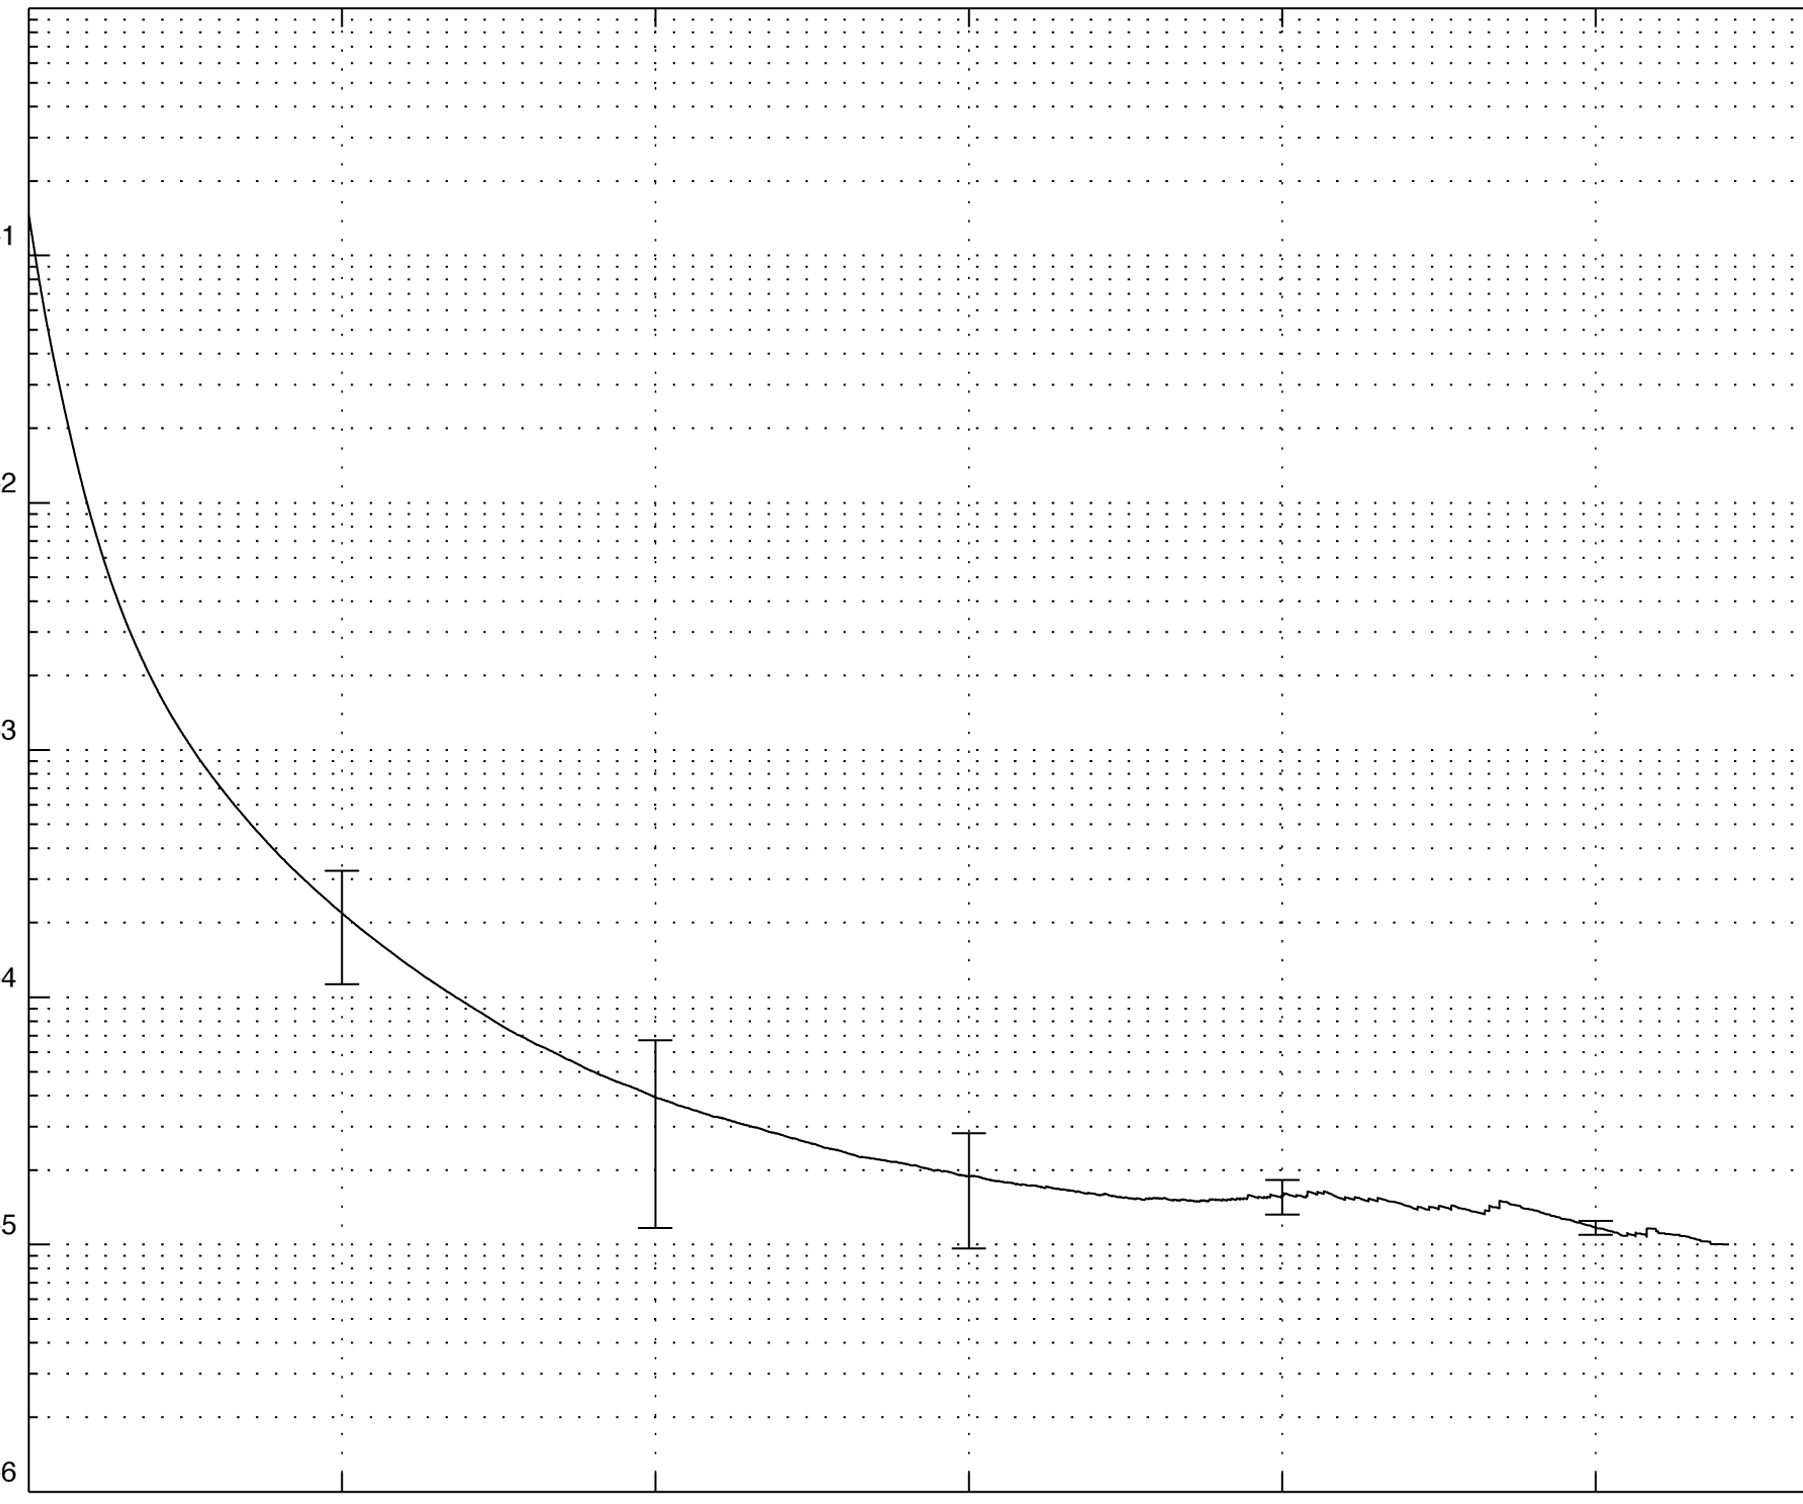
\includegraphics[width=.4\textwidth]{figure/hw2_curve.png} % width 
\caption{This an example curve. } % caption 
\label{hw2_fig1} % label 
\end{figure}

Figure 2 should contain two curves -- training error 
and testing error versus different numbers of training 
instances (thus x-axis is percentage of instances for 
training, and y-axis is prediction error). You need to 
try these percentages: 1\%, 5\%, 10\%, 20\%, 50\%, 75\%. 
Requirements of this figure are the same as for Figure
\ref{hw2_fig1}. 




\end{document}
